% ==================================================================
%  PageRank on a Toy Web Graph — Beamer slide deck (FIXED VERSION)
% ==================================================================
\documentclass{beamer}

% ----------------------------
%  Beamer theme & packages
% ----------------------------
\usetheme{Madrid}
\usepackage{tikz}
\usepackage{pgfplots}
\pgfplotsset{compat=1.18}
\usetikzlibrary{arrows.meta, positioning}
\usepackage{minted}    % syntax‑highlighted code blocks (needs -shell-escape)
\usepackage{booktabs}  % professional tables
\usepackage{amsmath}   % align*, \operatorname, etc.

% ----------------------------
%  Metadata
% ----------------------------
\title{PageRank on a Toy Web Graph}
\author{Emirhan Atar}
\institute{Discrete Mathematics II — 2025S}
\date{\today}

\begin{document}

% =======================================================
%  Title slide
% =======================================================
\begin{frame}
\titlepage
\end{frame}

% -------------------------------------------------------
%  Slide 1 — What is PageRank?
% -------------------------------------------------------
\begin{frame}{What is PageRank?}
\begin{itemize}
  \item Algorithm that assigns each node in a directed graph an \emph{importance probability}.  The vector of probabilities sums to~1.
  \item A hyperlink from page $u$ to page $v$ is treated as a “vote” for~$v$’s relevance.
  \item Votes from highly ranked pages weigh more than votes from low‑ranked ones — a recursive notion solved via linear algebra.
  \item Equivalent to the \textbf{stationary distribution} of a \emph{random surfer} who
  \begin{itemize}
    \item with probability $d$ follows an outgoing link, and
    \item with probability $1-d$ teleports to a random page.
  \end{itemize}
  \item Teleportation together with a special treatment of \emph{dangling pages} (pages with no out‑links) guarantees the underlying Markov chain is irreducible and aperiodic, so a unique stationary distribution exists.
  \item Invented by Larry Page and Sergey Brin (1998) and famously powered early Google Search.
\end{itemize}
\end{frame}

% -------------------------------------------------------
%  Slide 2 — Why PageRank?
% -------------------------------------------------------
\begin{frame}{Why PageRank?}
\begin{itemize}
  \item \textbf{Need for ranking:} The Web contains billions of pages; users expect the \emph{best} answers at the top of their query results.
  \item \textbf{Beyond keywords:} Early search engines ranked pages only by term frequency. Easy to game via keyword stuffing.
  \item \textbf{Link structure as a quality signal:} A page cited (linked) by many other pages—especially authoritative ones—tends to be more trustworthy and useful.
  \item \textbf{Mathematically principled:} Computes the stationary distribution of a Markov chain—guaranteed to converge under mild conditions.
  \item \textbf{Scalable \& incremental:} Power‑iteration is embarrassingly parallel; PageRank can be updated as the web evolves.
  \item \textbf{Versatile:} Variants appear in social‑network influence, recommendation systems, citation analysis, and bio‑informatics.
\end{itemize}
\end{frame}

% -------------------------------------------------------
%  Slide 3 — Algorithm Overview
% -------------------------------------------------------
\begin{frame}[fragile]{PageRank Algorithm — Overview}
\textbf{Recap idea}: iteratively redistribute score until it stabilises.

\begin{enumerate}
  \item \textbf{Initialise} each page $P_i$ with equal rank $PR(P_i)=1/N$.
  \item \textbf{Iterate} until convergence:
    \begin{enumerate}
      \item For every page $P_i$ compute the new rank
      \[
        PR_{\text{new}}(P_i) = \frac{1-d}{N}
          + d \sum_{P_j \rightarrow P_i} \frac{PR(P_j)}{\operatorname{outdeg}(P_j)}
          + d\,\frac{S_{\text{dangling}}}{N},
      \]
      where $S_{\text{dangling}}$ is the total rank currently sitting on pages with no out‑links.
      \item Replace $PR(P_i) \leftarrow PR_{\text{new}}(P_i)$ for all~$i$.
    \end{enumerate}
  \item \textbf{Stop} when the $\ell_1$ change $\sum_i |PR_{\text{new}}(P_i)-PR(P_i)|$ is below a tolerance~$\varepsilon$.
\end{enumerate}
\end{frame}

% -------------------------------------------------------
%  Slide 4 —  Pseudocode
% -------------------------------------------------------
\begin{frame}[fragile]{PageRank Algorithm — Reference Python}
\vspace{-0.7em}
\begin{minted}[fontsize=\tiny, linenos]{python}
from collections import defaultdict

def pagerank(graph, d=0.85, tol=1e-6, max_iter=100):
    """Return PageRank vector as a dict {node: score}.  graph is
    {u: [v1, v2, ...]} with an empty list for dangling pages."""
    N = len(graph)
    pr = {v: 1 / N for v in graph}

    # Pre-compute inbound links for O(V+E) per iteration
    in_links = defaultdict(list)
    for u, outs in graph.items():
        for v in outs:
            in_links[v].append(u)

    for _ in range(max_iter):
        dangling_sum = sum(pr[u] for u, outs in graph.items() if len(outs) == 0)

        new = {}
        for v in graph:
            rank_from_links = sum(pr[u] / len(graph[u]) for u in in_links[v])
            new[v] = (1 - d) / N + d * (rank_from_links + dangling_sum / N)

        # ℓ1 distance between successive vectors
        if sum(abs(new[v] - pr[v]) for v in pr) < tol:
            pr = new  # keep the most up‑to‑date vector
            break
        pr = new
    return pr
\end{minted}
\vspace{-0.3em}
\textit{Complexity}: $\mathcal{O}\big(k\,(V+E)\big)$ where $k$ is the number of iterations (\(k\approx50\) for $\varepsilon=10^{-6}$ on small graphs).
\end{frame}

% -------------------------------------------------------
%  Slide 5 — Example Calculation on Toy Graph
% -------------------------------------------------------
\begin{frame}{Example Calculation on a 5‑page Web}
\begin{columns}[T,totalwidth=\textwidth]
  \begin{column}{0.45\textwidth}
  \centering
  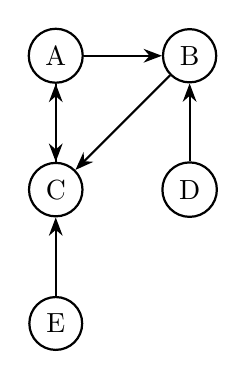
\begin{tikzpicture}[->,>=Stealth, node distance=1.7cm, thick]
    \node[circle,draw] (A) {A};
    \node[circle,draw, right of=A] (B) {B};
    \node[circle,draw, below of=A] (C) {C};
    \node[circle,draw, below of=B] (D) {D};
    \node[circle,draw, below of=C] (E) {E};

    \draw (A) -- (B);
    \draw (A) -- (C);
    \draw (B) -- (C);
    \draw (C) -- (A);
    \draw (D) -- (B);
    \draw (E) -- (C);
  \end{tikzpicture}
  \end{column}
  \begin{column}{0.55\textwidth}
  \small
  Damping factor $d=0.85$, $N=5$, initialise $PR^{(0)}=1/N=0.20$.

  \medskip
  \begin{tabular}{lcc}
    \toprule
    Page & $PR^{(0)}$ & $PR^{(1)}$ \\\midrule
    A & 0.20 & 0.20 \\
    B & 0.20 & 0.285 \\
    C & 0.20 & 0.455 \\
    D & 0.20 & 0.030 \\
    E & 0.20 & 0.030 \\\bottomrule
  \end{tabular}

  \medskip
  \begin{itemize}
    \item Total $\ell_1$ change $\|\Delta_1\|_1 = 0.68$.
    \item Largest per‑page change $\max_i |\Delta_{1,i}| = 0.255$ (page~C).
  \end{itemize}
  \end{column}
\end{columns}
\end{frame}

% -------------------------------------------------------
%  Slide 6 — Convergence plot
% -------------------------------------------------------
\begin{frame}{Convergence of PageRank Values}
\centering
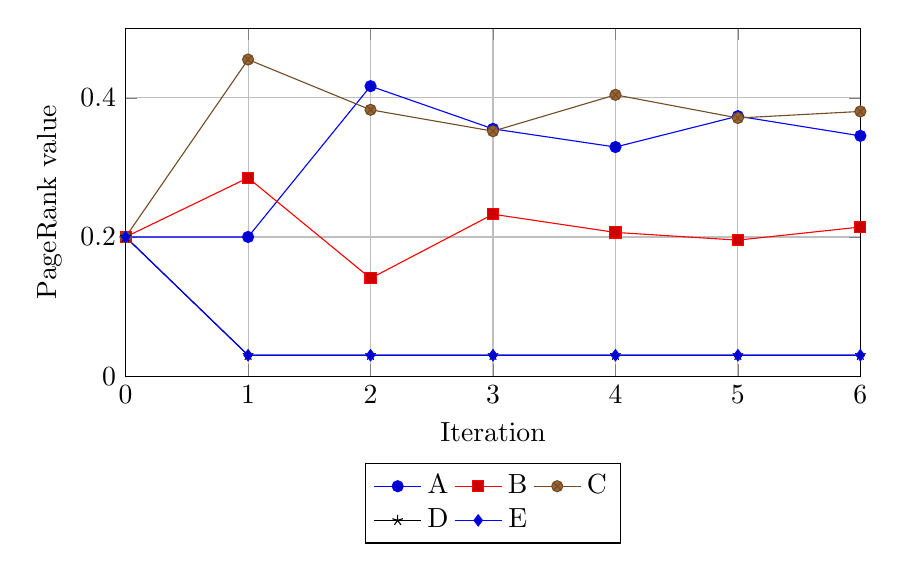
\begin{tikzpicture}
  \begin{axis}[
    width=0.9\linewidth,
    height=6cm,
    xlabel={Iteration}, ylabel={PageRank value},
    ymin=0,ymax=0.5,
    xmin=0,xmax=6,
    legend style={at={(0.5,-0.25)},anchor=north,legend columns=3},
    grid=both,
  ]
    % Page A
    \addplot coordinates {(0,0.20) (1,0.20) (2,0.41675) (3,0.35534) (4,0.32924) (5,0.37361) (6,0.34532)}; \addlegendentry{A}
    % Page B
    \addplot coordinates {(0,0.20) (1,0.285) (2,0.1405) (3,0.23262) (4,0.20652) (5,0.19543) (6,0.21428)}; \addlegendentry{B}
    % Page C
    \addplot coordinates {(0,0.20) (1,0.455) (2,0.38275) (3,0.35204) (4,0.40424) (5,0.37097) (6,0.38040)}; \addlegendentry{C}
    % Page D
    \addplot coordinates {(0,0.20) (1,0.03) (2,0.03) (3,0.03) (4,0.03) (5,0.03) (6,0.03)}; \addlegendentry{D}
    % Page E
    \addplot coordinates {(0,0.20) (1,0.03) (2,0.03) (3,0.03) (4,0.03) (5,0.03) (6,0.03)}; \addlegendentry{E}
  \end{axis}
\end{tikzpicture}

\vspace{0.35em}
\small
Ranks stabilise in roughly six iterations \emph{for this five‑page graph}.  Pages~D and~E have no incoming links, so after the first round they keep the teleportation baseline $0.03$.
\end{frame}

% -------------------------------------------------------
%  Slide 7 — Real‑World Impact of PageRank
% -------------------------------------------------------
\begin{frame}{Real‑World Impact of PageRank}
\begin{itemize}
  \item \textbf{Google Search:} PageRank was a foundational algorithm in Google Search, ranking pages based on their link structure.
  \item \textbf{Academic Citations:} Used to rank scientific papers, helping to measure the influence of a paper or author.
  \item \textbf{Social Networks:} Applied to rank individuals or posts in social media platforms based on connections or influence.
  \item \textbf{Recommendation Systems:} PageRank principles can rank products or content based on user interactions (e.g., Amazon or YouTube recommendations).
\end{itemize}
\end{frame}

% -------------------------------------------------------
%  Slide 8 — Summary & Takeaways
% -------------------------------------------------------
\begin{frame}{Summary & Takeaways}
\begin{itemize}
  \item \textbf{PageRank Algorithm:} A Markov‑chain method for ranking web pages based on their link structure and the importance of incoming links.
  \item \textbf{Convergence:} For our toy five‑page graph, PageRank values converge after about six iterations with $d=0.85$ and $\varepsilon=10^{-6}$.  Larger or denser graphs typically need dozens of iterations.
  \item \textbf{Real‑World Applications:} From Google Search to academic citation rankings, PageRank has a significant impact across multiple domains.
\end{itemize}
\vspace{1em}
\centering
\end{frame}

\end{document}
